% !TeX root = ../Masterarbeit.tex
\graphicspath{{kap03/figures/}{./figures/}}
\section{Chance Constraints and Kernel Density Estimation}
\label{ch:kde}

Chapter~2 surveyed the optimization paradigms and approximation methods that motivate a nonparametric treatment of chance constraints. This chapter narrows that survey to kernel density estimation (KDE): it defines the residual-space estimator, explains bandwidth and dimensionality trade-offs, and maps the relevant chance-constraint literature to the gap addressed by the thesis. Chapter~4 then derives the smooth residual-KDE reformulation used in the optimization experiments.

\subsection{Kernel density estimation for residual probabilities}
\label{sec:kde}

\subsubsection{Parzen--Rosenblatt estimator and residual CDF}
\label{ssec:parzen}

Let $y_1(x),\ldots,y_N(x)$ be IID residual samples and let $\rho_x$ denote the density of $Y(x)=g(x,\xi)$, assumed to exist for the decisions under study. For a nonnegative kernel $K$ with $\int K(u)\,du=1$ and bandwidth $h>0$, the KDE is
\begin{equation}
 \hat\rho_h(y;x)=\frac{1}{Nh}\sum_{i=1}^N K\!\left(\frac{y-y_i(x)}{h}\right),
 \qquad
 \hat p_h(x)=\int_{-\infty}^{0}\hat\rho_h(y;x)\,dy.
 \label{eq:ch3-kde}
\end{equation}
This is the Parzen--Rosenblatt estimator~\citep{rosenblatt1956,parzen1962}. If $F_K(t)=\int_{-\infty}^tK(u)\,du$, then $\hat p_h(x)=N^{-1}\sum_iF_K(-y_i(x)/h)$. Thus the probability is a finite sum of integrated-kernel evaluations rather than a numerical integral over uncertainty space. For IID samples and a regular residual density (for example, the usual smoothness and integrability conditions on $\rho_x$), pointwise consistency uses a bandwidth sequence $h_N$ satisfying $h_N\to0$ and $Nh_N\to\infty$~\citep{parzen1962,devroye1985}. The sequence links smoothing to sample size: the normal-reference rule introduced below chooses $h_N=O(N^{-1/5})$. This is pointwise/statistical consistency for a fixed decision and does not by itself imply convergence of a data-selected optimizer; optimizer convergence requires stronger uniform convergence and optimization regularity, as discussed in Section~\ref{ssec:safetyline}.

The uncertainty sample is drawn once and kept fixed during optimization, while $y_i(x)=g(x,\xi_i)$ changes at every iterate. This preserves a deterministic sample problem and permits differentiation through the residual map. With fixed $h$ and continuous $K$, the integrated estimate is continuously differentiable wherever $g$ is continuously differentiable; a continuously differentiable kernel supports a second derivative when the residual also has the required regularity. Thus a kernel need not itself be infinitely smooth to provide a differentiable probability constraint.

The statistical and computational roles of the estimator are different. One scalar chance constraint becomes one aggregated inequality, but its evaluation and gradient still require $N$ residual contributions. Residual scalarization reduces the dimension of the density estimate; it does not make simulation cost independent of sample size. Chapter~4 makes these costs explicit when deriving the gradient and assembling the nonlinear program.

\subsubsection{Kernel choices and one-sided bias}
\label{ssec:kernels}

The Gaussian kernel is infinitely differentiable and has $F_K=\Phi$. The compactly supported Epanechnikov kernel, $K(u)=\tfrac34(1-u^2)_+$, is efficient for classical density estimation~\citep{epanechnikov1969}. Both are symmetric: their integrated functions smooth the indicator from both sides and can overestimate the safe probability. The Split--Bernstein constructions of Keil et al. are designed for a one-sided safety property~\citep{keil2020,keil2021}. The local implementation in this thesis uses a shifted Epanechnikov analogue and does not reproduce the published Split--Bernstein/MCMC/optimal-control workflow. A pointwise kernel inequality for a fixed decision is therefore distinct from a finite-sample guarantee for the optimized decision.

For the safe-probability convention used here, a fully shifted compact kernel gives a simple illustration. With the Epanechnikov CDF $F_K$ and shift $b(h)=h$, the per-sample contribution is
\begin{equation}
 s_h(y)=F_K\!\left(\frac{-y-h}{h}\right)
 \leq\ind\{y\leq0\}.
 \label{eq:ch3-kernel-envelope}
\end{equation}
Consequently, the smoothed safe fraction is bounded by the empirical safe fraction for every fixed sample. Taking expectations at a fixed decision gives a lower bound on the population safe probability. Neither statement removes random sampling error at a decision selected using that sample. Figure~\ref{fig:kernels} displays the underlying integrated-kernel inequality using a standardized argument.

\begin{figure}[t]
  \centering
  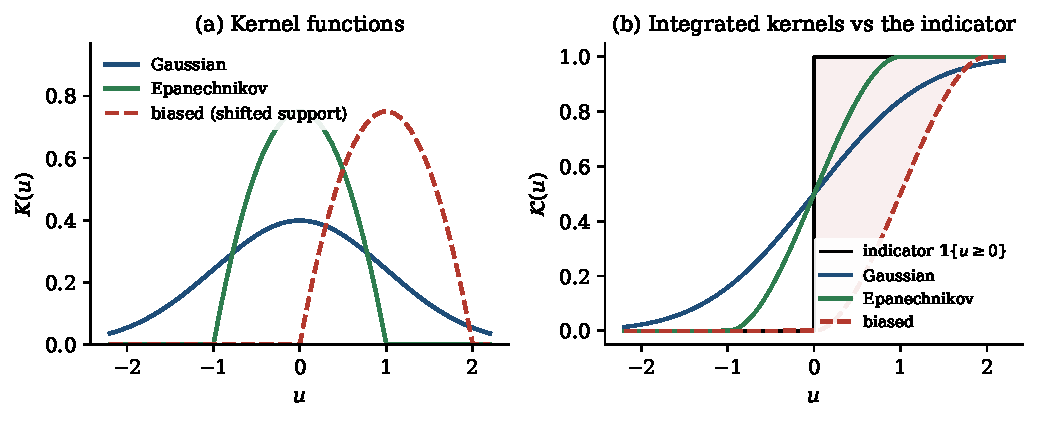
\includegraphics[width=\textwidth]{fig_kernels.pdf}
  \caption{Kernel shapes and integrated kernels. The shifted Epanechnikov kernel has support $[0,2]$ in the standardized argument, so its CDF is bounded above by $\ind\{u\geq0\}$. This is a per-sample smoothing inequality. It does not by itself give a finite-sample population guarantee for a data-selected decision.}
  \label{fig:kernels}
\end{figure}

\subsubsection{Bandwidth and AMISE}
\label{ssec:bandwidth}

Bandwidth controls the bias--variance trade-off. For a twice-differentiable density $\rho_x$, define $R(\phi)=\int\phi(u)^2du$ and $\mu_2(K)=\int u^2K(u)\,du$. The standard one-dimensional expansion is
\begin{equation}
 \operatorname{AMISE}(h)=\frac{R(K)}{Nh}+\frac{h^4\mu_2(K)^2}{4}R(\rho_x''),
 \label{eq:ch3-amise}
\end{equation}
with optimal order $h=O(N^{-1/5})$ and error $O(N^{-4/5})$~\citep{silverman1986}. Silverman's and Scott's rules, plug-in estimates, and cross-validation estimate the unknown scale or curvature term~\citep{silverman1986,scott1992,wand1995}. They minimize a density-estimation criterion, however. In this thesis the KDE is thresholded at zero, differentiated through $g(x,\xi_i)$, and embedded in an optimizer; the bandwidth that minimizes AMISE need not minimize objective error, constraint error, or tail error. Figure~\ref{fig:bandwidth} illustrates the density-level bias--variance trade-off used to motivate the optimization sensitivity study.

\begin{figure}[t]
  \centering
  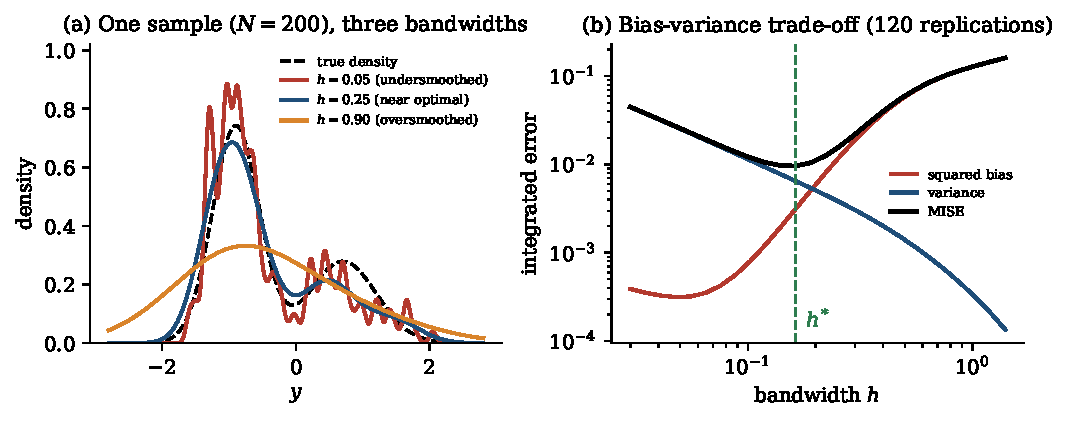
\includegraphics[width=0.82\textwidth]{fig_bandwidth.pdf}
  \caption{Bandwidth trade-off for a seeded bimodal density reconstruction. (a) Small bandwidth follows sample noise, an intermediate bandwidth recovers the two modes, and large bandwidth blurs them. (b) Across 120 replications, variance decreases and squared bias increases with bandwidth; their sum has an interior minimum. The plot concerns density error, so its minimizer need not be optimal for a chance-constrained decision.}
  \label{fig:bandwidth}
\end{figure}

In practice, the bandwidth is selected jointly with the sample size rather than held fixed across the asymptotic sequence. For example, the robust normal-reference rule commonly attributed to Silverman is
\begin{equation}
 h_N=0.9\min\{\widehat\sigma,\operatorname{IQR}/1.34\}N^{-1/5},
 \label{eq:ch3-bandwidth-rule}
\end{equation}
where $\widehat\sigma$ and the interquartile range measure sample scale~\citep{silverman1986}. A normal-reference constant is an initialization choice, not evidence that a multimodal or heavy-tailed residual is Gaussian. Cross-validation and plug-in procedures use different criteria and can select different bandwidths. If the bandwidth is recomputed as the decision changes, its dependence must also be accounted for in the derivatives or explicitly frozen; the formula in Chapter~4 assumes a fixed bandwidth during that differentiation.

Tail constraints require additional care even in one dimension. A sample contains on average $N\varepsilon$ observations in an event of probability $\varepsilon$, so a small violation budget can be weakly resolved despite a visually smooth density. Density-integrated error also weights regions differently from a constraint evaluated at one threshold. The experiments therefore report bandwidth, sample size, and held-out event frequency together instead of interpreting a favorable density plot as a reliability certificate.

\subsubsection{Multivariate KDE and residual scalarization}
\label{ssec:curse}

For a $d$-dimensional variable, a bandwidth matrix $H$ gives
\begin{equation*}
  \widehat f_H(y)=\frac{1}{N}\sum_{i=1}^N |H|^{-1/2} K\!\left(H^{-1/2}(y-y_i)\right).
\end{equation*}
The optimal error rate becomes $O(N^{-4/(d+4)})$, with bandwidth order $O(N^{-1/(d+4)})$~\citep{silverman1986,scott1992}. Holding accuracy fixed therefore requires rapidly increasing sample size. Figure~\ref{fig:curse} plots the rate-based sample requirement normalized to $N=100$ in one dimension; its values are illustrations from the rate, not measured minimum sample sizes.

The residual-space construction avoids estimating the full $d$-dimensional uncertainty law for an individual constraint. It estimates the scalar $Y(x)=g(x,\xi)$ and integrates over the fixed half-line $(-\infty,0]$. This removes the uncertainty dimension from the KDE itself, but not from sampling or simulation. A joint constraint has a residual vector of dimension $m$; a scalar maximum preserves one-dimensional estimation but introduces a non-smooth maximum, while multivariate residual KDE reintroduces the dimensionality cost. Chapter~5 compares these alternatives.

\begin{figure}[t]
  \centering
  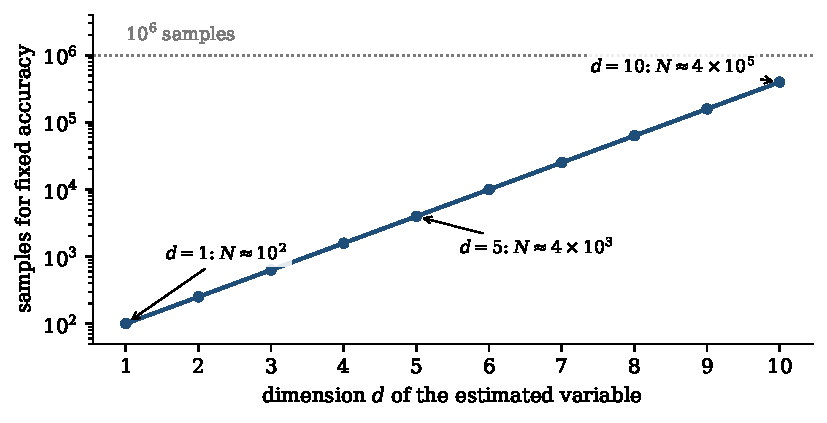
\includegraphics[width=0.8\textwidth]{fig_curse.pdf}
  \caption{Rate-based illustration of the curse of dimensionality. The plotted sample count is the order required to retain the accuracy of $N=100$ samples in one dimension under the AMISE rate $O(N^{-4/(d+4)})$. The annotations are approximate scaling values, not empirical requirements for a particular application.}
  \label{fig:curse}
\end{figure}

\subsection{KDE in the chance-constrained literature}
\label{sec:litmap}

\subsubsection{Application streams}
\label{ssec:firstwave}

An early practical use of kernel-smoothed chance constraints replaced a specified process-planning distribution with historical data~\citep{calfa2015}. The same residual-probability construction was subsequently used in aerospace optimal control for launcher ascent and the Goddard problem~\citep{caillau2018}. Energy-system work developed adaptive KDE formulations for microgrids and extended them to dispatch and power-system scheduling with multivariate or joint constraints~\citep{ciftci2017,ciftci2019,wu2021,wu2023}. These streams establish practical breadth, but their guarantees are primarily estimator-level.

The application papers do not all estimate the same object or provide the same guarantee. Calfa et al. treat individual and joint constraints with right-hand-side uncertainty using kernel-smoothed univariate quantiles and multivariate distribution functions, together with a divergence-based treatment of distributional uncertainty~\citep{calfa2015}. The optimal-control line uses kernel probability approximations inside trajectory optimization, where derivative availability and transcription accuracy become central~\citep{caillau2018,keil2021}. The energy and network papers demonstrate settings in which empirical disturbance distributions and coupled constraints are relevant. Their results motivate the model adapters in this thesis, but are not reproduced merely by applying a scalar estimator to a synthetic residual.

\subsubsection{Safety-oriented kernels and convergence theory}
\label{ssec:safetyline}

Keil et al. introduced biased kernels whose integrated functions are constructed to lie on the conservative side of the violation indicator and applied them to chance-constrained soft lunar landing~\citep{keil2020,keil2021}. A warm-start continuation strategy reduces the numerical cost of changing bandwidth and kernel bias~\citep{keil2021warm}. Network applications and analytic-gradient treatments further demonstrate that the construction is not limited to one domain~\citep{gugat2018,schuster2022}. Adjacent work studies nonparametric prediction intervals, distributionally robust load shedding, portfolio tail risk, and kernel embeddings in robotics~\citep{wan2020,wang2021,qi2026,liu2022,gopalakrishnan2018}.

KDE consistency alone concerns the estimated probability for a fixed decision. Schuster's optimizer-level results establish convergence of optimal values and solution sets under explicit assumptions on the residual density, kernel, bandwidth sequence, uniform convergence, and the optimization problem~\citep{schuster2025}. They are asymptotic results, not finite-sample confidence bounds. The unresolved practical boundary addressed here is the connection between these assumptions and nonlinear numerical programs: how bandwidth choices behave inside an optimizer, how a one-sided local surrogate affects cost and held-out violations, and how joint-event reductions change the measured risk. Chapters~4--6 develop the formulation and its qualifications; Chapters~7--9 test the resulting evidence chain on declared synthetic models.

\begin{figure}[t]
  \centering
  
\includegraphics[width=0.88\textwidth]{fig_litmap.pdf}
  \caption{Condensed path from analytical chance constraints to data-driven residual KDE. The literature spans process systems, aerospace, energy and network applications, safety-oriented biased kernels, and optimizer-level convergence theory. The thesis studies their connection under explicit finite-sample and implementation qualifications.}
  \label{fig:litmap}
\end{figure}
